\documentclass[svgnames,x11names,dvipsnames]{beamer}
% --- Self-contained preamble (same conventions as the course decks).
% --- If you prefer, replace this block with \input{preamble}.
\usepackage[utf8]{inputenc}
\usepackage[T1]{fontenc}
\usepackage[english]{babel}
\usepackage{amsmath,amssymb}
\usepackage{xcolor}
\usepackage{graphicx}
\usepackage{hyperref}
\usepackage{booktabs}
\usepackage{array}
\IfFileExists{lmodern.sty}{\usepackage{lmodern}}{}
\usepackage{tikz}
\usetikzlibrary{positioning,arrows.meta,calc,fit,decorations.pathreplacing}
\usepackage[font=footnotesize]{caption}
\usepackage{qrcode}
\usepackage{eurosym}

\definecolor{color1bg}{HTML}{005e9e}
\setbeamercolor*{palette primary}{fg=white,bg=color1bg}
\setbeamercolor*{block title}{bg=color1bg,fg=white}
\setbeamercolor*{frametitle}{fg=color1bg}
\setbeamertemplate{caption}[numbered]
\definecolor{color2bg}{HTML}{003a63}
\setbeamercolor{block title alerted}{bg=color2bg,fg=white}
\setbeamercolor{block body alerted}{bg=color2bg!8}
\setbeamercolor{alerted text}{fg=color2bg}
\beamertemplatenavigationsymbolsempty

% --- Slide numbers on every slide except the title page.
\setbeamertemplate{background}{%
  \ifnum\value{page}>1
    \begin{tikzpicture}[remember picture,overlay]
      \node[anchor=south east,font=\fontsize{7}{8}\fontfamily{lmr}\fontseries{l}\selectfont,text=gray!80] at ([xshift=-0.3cm,yshift=0.2cm]current page.south east) {\insertpagenumber};
    \end{tikzpicture}%
  \fi}

% --- This deck: one blue everywhere, the blue of the title page (Beamer's default, #3333B2).
% --- Delete this block to go back to color1bg / color2bg.
\definecolor{titleblue}{HTML}{3333B2}
\definecolor{accentred}{HTML}{B22222}
\colorlet{color1bg}{titleblue}
\colorlet{color2bg}{titleblue!75!black}
\setbeamercolor*{frametitle}{fg=titleblue}
\setbeamercolor*{block title}{bg=titleblue,fg=white}
\setbeamercolor{block title alerted}{bg=titleblue,fg=white}
\setbeamercolor{block body alerted}{bg=titleblue!8}
\setbeamercolor{alerted text}{fg=titleblue}

% --- Change marker, as in the other decks: wrap a change in \chg{...} to see it in bold.
% --- Switched off; comment the second line to see the changes.
\newcommand{\chg}[1]{{\bfseries #1}}
\renewcommand{\chg}[1]{#1}

\newcommand{\sectionslide}[2]{%
\begin{frame}[plain]
  \centering
  \vfill
  {\LARGE \textbf{\textcolor{titleblue}{#1}}}\\[0.4cm]
  {#2}
  \vfill
\end{frame}}

\title[LLMs for Social Science Research]{\large \textbf{Large Language Models for Social Science Research} \\
    \textit{Session 4. From Texts to Variables, With and Without an LLM}}
\author[H. Subtil]{\textbf{Hugo Subtil}}
\institute{PhD Workshop, University of Zurich}
\date{November 18, 2026}

\begin{document}
\frame{\titlepage}

\begin{frame}{Course Repository}
\centering
\vspace{0.2cm}
\qrcode[height=3.6cm]{https://github.com/subtilhugo/uzh-llm-socsci-2026}

\vspace{0.5cm}
{\large \href{https://github.com/subtilhugo/uzh-llm-socsci-2026}{\texttt{github.com/subtilhugo/uzh-llm-socsci-2026}}}

\vspace{0.4cm}
{\small Download it again: \texttt{sessions/04/} and prompts 12 to 14.}
\end{frame}

\begin{frame}{Today's Session Overview (9:00--12:00)}

\setlength{\leftmargini}{2.3cm}
\small
\begin{enumerate}
    \setlength{\itemsep}{1pt}
    \item[\textbf{9:00--9:10}] Last Week, and the Question We Left Open

    \item[\textbf{9:10--9:45}] Part 1. The ScienceCluster, for Real
    \begin{itemize}
        \item SSH: build, fetch, submit a GPU job
        \item The browser: ScienceApps, the same environment
    \end{itemize}

    \item[\textbf{9:45--10:40}] Part 2. Measuring Without an LLM, then a break
    \begin{itemize}
        \item Block 1. Collect, and code six documents by hand
        \item Block 2. A dictionary, embeddings, a classifier (12)
    \end{itemize}

    \item[\textbf{10:50--11:30}] Part 3. Extracting With an LLM
    \begin{itemize}
        \item Block 3. Claude and GPT fill in a form, checked against the catalogue (13)
    \end{itemize}

    \item[\textbf{11:30--11:50}] Part 4. From Labels to an Estimate
    \begin{itemize}
        \item Block 4. The coefficient, naive and corrected (14)
    \end{itemize}

    \item[\textbf{11:50--12:00}] Debrief and Next Session
\end{enumerate}
\end{frame}

\begin{frame}{Last Week, and the Question We Left Open}
\small
\textbf{The method.} A data API, with a number you did not produce. A model API, with a codebook and a schema. A local model, with its digest.

\vspace{0.3cm}
\textbf{The result.} On 34 manifestos, GPT said ``yes'' far more often than the dictionaries on the local offer and on class conflict. Neither is ground truth: a disagreement is a passage to read.

\vspace{0.7cm}
\centering
\alert{The model agrees with the human coders on 75\% of the documents.\\ Your regression uses its labels. What would you have to show\\ for a referee to accept the coefficient?}
\end{frame}

\begin{frame}{Today's Question}
\small
\textbf{Do candidates who already hold a local office talk more about local issues?}

\vspace{0.3cm}
The professions de foi of the first round of the 1978 legislative election: 4,010 documents in Archelec (Sciences Po, CEVIPOF). We draw 300.

\vspace{0.4cm}
\renewcommand{\arraystretch}{1.4}
\begin{tabular}{@{}>{\raggedright\arraybackslash}p{2.6cm}>{\raggedright\arraybackslash}p{7.6cm}@{}}
\toprule
\textbf{Y} \newline {\scriptsize a local offer} & by hand (Part 2), a dictionary, embeddings, a classifier (Part 2), Claude and GPT (Part 3) \\
\textbf{X} \newline {\scriptsize a local office} & the catalogue of Sciences Po, and the same variable extracted by the LLMs (Part 3) \\
\textbf{The estimate} & naive, and corrected with your hand codes (Part 4) \\
\bottomrule
\end{tabular}

\vspace{0.4cm}
\centering
\alert{Six ways to measure Y. One coefficient. Which one do you print?}
\end{frame}

% ============================================================================
\sectionslide{Part 1. The ScienceCluster, for Real}{One task, two doors}

\begin{frame}{Why Now}
\small
Last time, the doors. Today, a task that needs them: \textbf{embed the 4,010 professions de foi of 1978}, then work on them in a notebook.

\vspace{0.4cm}
\renewcommand{\arraystretch}{1.4}
\footnotesize
\begin{tabular}{@{}>{\raggedright\arraybackslash}p{2.4cm}>{\raggedright\arraybackslash}p{2.4cm}>{\raggedright\arraybackslash}p{2.4cm}>{\raggedright\arraybackslash}p{2.8cm}@{}}
\toprule
& \textbf{Your laptop} & \textbf{Colab} & \textbf{ScienceCluster} \\
\midrule
GPU & yours, if any & a free T4, for a while & L4, A100, H100, H200 \\
How long & while it is on & a few hours & up to 7 days \\
Where the data go & nowhere & Google's machines & nowhere: UZH \\
Who pays & you & free tier, or a plan & your group's project \\
\bottomrule
\end{tabular}

\vspace{0.4cm}
\small
\textbf{Access}: your group's Science IT project; your PI adds you. VPN off campus.
\end{frame}

\begin{frame}{Today's Task}
\centering
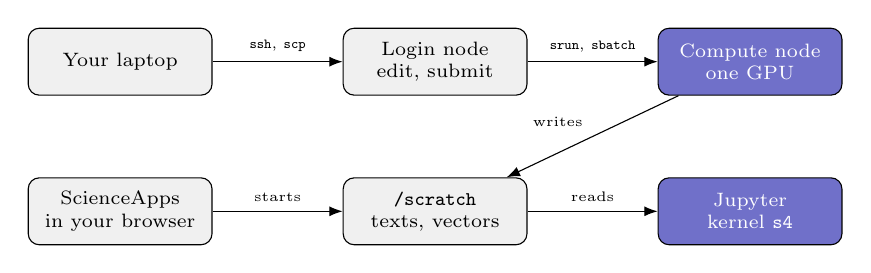
\begin{tikzpicture}[font=\scriptsize]
  \tikzset{box/.style={draw,rounded corners,minimum height=0.85cm,text width=2.1cm,align=center,fill=gray!12},
           key/.style={draw,rounded corners,minimum height=0.85cm,text width=2.1cm,align=center,fill=titleblue!70,text=white}}
  \node[box] (lap) at (0,0) {Your laptop};
  \node[box] (login) at (4,0) {Login node\\edit, submit};
  \node[key] (gpu) at (8,0) {Compute node\\one GPU};
  \node[box] (apps) at (0,-1.9) {ScienceApps\\in your browser};
  \node[box] (scratch) at (4,-1.9) {\texttt{/scratch}\\texts, vectors};
  \node[key] (jup) at (8,-1.9) {Jupyter\\kernel \texttt{s4}};
  \draw[-{Latex}] (lap) -- node[above,font=\tiny]{\texttt{ssh}, \texttt{scp}} (login);
  \draw[-{Latex}] (login) -- node[above,font=\tiny]{\texttt{srun}, \texttt{sbatch}} (gpu);
  \draw[-{Latex}] (gpu) -- node[above left,font=\tiny]{writes} (scratch);
  \draw[-{Latex}] (apps) -- node[above,font=\tiny]{starts} (scratch.west);
  \draw[-{Latex}] (scratch) -- node[above,font=\tiny]{reads} (jup);
\end{tikzpicture}

\vspace{0.6cm}
\raggedright
\small
\begin{enumerate}
    \setlength{\itemsep}{3pt}
    \item Once: build one environment (a container) on a compute node.
    \item Fetch the corpus from the Internet Archive API, and check it.
    \item Submit the job: 4,010 documents embedded on one GPU.
    \item Open the notebook in ScienceApps, with the same environment, next to the vectors.
\end{enumerate}
\end{frame}

\begin{frame}[fragile]{Door 1. Once: One Environment}
\small
The S3IT way: no \texttt{pip install} on the cluster, a container built from a conda file.

\vspace{0.2cm}
{\scriptsize
\begin{verbatim}
# on your laptop
scp -r sessions/04/cluster <you>@cluster.s3it.uzh.ch:~/s4

ssh -l <you> cluster.s3it.uzh.ch
cd ~/s4
# building is work: on a compute node, not the login node
srun --pty -n 1 -c 2 --time=01:00:00 --mem=16G bash -l
module load apptainer
APPTAINER_BINDPATH="" apptainer build /scratch/$USER/s4.sif s4.def
\end{verbatim}}

\vspace{0.2cm}
\begin{columns}[T]
\column{0.45\textwidth}
\footnotesize
\texttt{env.yml}: pandas, scikit-learn, sentence-transformers, the Anthropic and OpenAI libraries, ipykernel.
\column{0.5\textwidth}
\footnotesize
\texttt{s4.def}: start from \texttt{miniforge3}, create the environment, put it on the \texttt{PATH}. Ten to twenty minutes, once.
\end{columns}
\end{frame}

\begin{frame}[fragile]{Door 1. Fetch the Corpus, and Check It}
\small
Still on the compute node. A data API again, with the same accounting as in Session 3.

\vspace{0.2cm}
{\scriptsize
\begin{verbatim}
curl -sI https://archive.org | head -1    # does this node reach out?
apptainer exec /scratch/$USER/s4.sif python fetch_corpus.py \
    --date 1978-03-12 --out /scratch/$USER/archelec
# 4010 documents found, 4010 to fetch
# requested 4010 = returned ... + missing ...

export HF_HOME=/scratch/$USER/hf           # the model, once, on scratch
apptainer exec /scratch/$USER/s4.sif python embed_corpus.py \
    --download-only
exit
\end{verbatim}}

\vspace{0.2cm}
Texts, model, vectors: on \texttt{/scratch}. Purged after 30 days unused, no backup. The texts are under a restrictive licence: never in a public repository.
\end{frame}

\begin{frame}[fragile]{Door 1. The Job}
\scriptsize
\begin{verbatim}
#!/usr/bin/bash -l
#SBATCH --job-name=embed-1978
#SBATCH --time=00:30:00
#SBATCH --cpus-per-task=4
#SBATCH --mem=16G
#SBATCH --gpus=1
#SBATCH --output=logs/%x_%j.out

module load apptainer
export HF_HOME=/scratch/$USER/hf
apptainer exec --nv /scratch/$USER/s4.sif python embed_corpus.py \
    --corpus /scratch/$USER/archelec/1978-03-12
\end{verbatim}

\vspace{0.2cm}
\begin{verbatim}
module load l4 && mkdir -p logs
sbatch embed.sbatch             # Submitted batch job 1234567
squeue --me                     # PD = waiting for a GPU, R = running
tail -f logs/embed-1978_1234567.out
\end{verbatim}

\vspace{0.1cm}
\small
\texttt{--nv} gives the container the GPU. The log ends with \texttt{run.json}: model, GPU, passages, seconds.
\end{frame}

\begin{frame}[fragile]{Door 3. The Same Environment in the Browser}
\small
\textbf{Once}: the container becomes a Jupyter kernel (S3IT's script).

{\tiny
\begin{verbatim}
curl -O https://gitlab.uzh.ch/s3it/docs/-/snippets/271/raw/main/apptainer_ipykernel.py
python apptainer_ipykernel.py install /scratch/$USER/s4.sif --name s4
\end{verbatim}}

\vspace{0.2cm}
\textbf{Every time}: \href{https://apps.s3it.uzh.ch}{\texttt{apps.s3it.uzh.ch}}
\begin{enumerate}
    \setlength{\itemsep}{2pt}
    \item Interactive Apps, Jupyter. Hours 3, cores 4, RAM 16 GB, GPU L4.
    \item My Interactive Sessions: Connect. Today's notebook, kernel \texttt{s4}.
    \item Keys in \texttt{\textasciitilde/.env} (\texttt{chmod 600}); \texttt{CLUSTER\_EMBEDDINGS} set to the job's folder.
    \item Delete the session when you are done: it is billed while it runs.
\end{enumerate}

\vspace{0.2cm}
No \texttt{pip install} in a cell: the container is fixed. A new package, a new build.
\end{frame}

\begin{frame}{Part 1. Follow Along}
\small
\textbf{I show.} The four steps, live. The job goes in at the start, and is done before the end of Part 1.

\vspace{0.4cm}
\textbf{You do}
\begin{itemize}
    \setlength{\itemsep}{4pt}
    \item \textbf{With an account}: \texttt{sessions/04/cluster/README.md}, step by step. Building takes time: start it now, come back to it at the break.
    \item \textbf{Without}: open today's notebook in Colab and run Part 0. Keep the README for the day you have an account.
\end{itemize}

\vspace{0.4cm}
\textbf{We check.} Shared document: the job ID, the GPU in the log, the seconds.

\vspace{0.4cm}
\textbf{An agent on the cluster} (Door 2) writes and resubmits job scripts well: \texttt{setup/cluster\_guide.md}.
\end{frame}

% ============================================================================
\sectionslide{Part 2. Measuring Without an LLM}{Words, geometry, a classifier}

\begin{frame}{The Data: Archelec}
\small
The electoral archive of Sciences Po (CEVIPOF): professions de foi and other electoral documents since 1958, on the Internet Archive. 36,843 documents.

\vspace{0.3cm}
\textbf{Per document}
\begin{itemize}
    \setlength{\itemsep}{3pt}
    \item The scan, and its OCR text (Tesseract).
    \item \textbf{A catalogue record} written by Sciences Po: the candidate, the substitute (\textit{suppl\'eant}), sex, profession, current offices, party support. ``NR'' = not recorded.
\end{itemize}

\vspace{0.3cm}
\textbf{The API}: a search (\texttt{advancedsearch}), a record (\texttt{metadata/<id>}), a text (\texttt{download/<id>/<id>\_djvu.txt}). No key.

\vspace{0.3cm}
\textbf{The terms}: CC BY-NC-ND, rights ``restricted''. Read them, share nothing in public.
\end{frame}

\begin{frame}{A Catalogue Record}
\footnotesize
Pas-de-Calais, 14th constituency, 1958, round 1.

\vspace{0.2cm}
\renewcommand{\arraystretch}{1.3}
\begin{tabular}{@{}lll@{}}
\toprule
& \textbf{Candidate} & \textbf{Substitute} \\
\midrule
Name & Legrand, Joseph & Six, Ren\'e \\
Sex & H & H \\
Profession & ouvrier surface & m\'ecanicien \\
Current office & NR & \textbf{maire} \\
Party support & Parti communiste fran\c{c}ais & Parti communiste fran\c{c}ais \\
Other & prisonnier de guerre & d\'eport\'e, famille nombreuse \\
\bottomrule
\end{tabular}

\vspace{0.4cm}
\small
Someone read the leaflet and filled in this form. Today an LLM fills in the same form, and we compare.

\vspace{0.3cm}
\centering
\alert{The mayor is the substitute, not the candidate:\\ exactly the confusion a model must avoid.}
\end{frame}

\begin{frame}{Block 1. Collect, and Code by Hand}
\small
\textbf{I show.} Notebook, Parts 1 and 2: the search, the draw of 300, the checks, the catalogue.

\vspace{0.3cm}
\textbf{You do}
\begin{enumerate}
    \setlength{\itemsep}{3pt}
    \item Notebook Part 1: read the checks: found, requested, returned, missing, empty.
    \item \texttt{MY\_NUMBER}: the number next to your name in my email.
    \item Code \textbf{six documents}: the common one, then your five. Read the PDF. One definition:
\end{enumerate}

{\footnotesize
\textit{local\_offer: a geographically specific local issue, institution, project, service, firm, infrastructure, place, or population. A candidate name, constituency heading, or place name alone is insufficient.}}

\vspace{0.2cm}
\begin{enumerate}
    \setcounter{enumi}{3}
    \item Paste your six lines in the shared sheet.
\end{enumerate}

\vspace{0.2cm}
\textbf{We check.} The common document: how many of you said yes?
\end{frame}

\begin{frame}{Why Your Six Codes Matter}
\small
The documents were handed out in an order drawn at random. So the documents you coded are \textbf{a random sample} of the 300, and each had \textbf{a known probability} of being coded:

\[
\pi = \frac{\text{documents coded by the class}}{300}
\]

\vspace{0.3cm}
\begin{itemize}
    \setlength{\itemsep}{4pt}
    \item Part 2: the reference for every measure.
    \item Part 4: what makes the coefficient correctable.
\end{itemize}

\vspace{0.4cm}
\centering
\alert{A gold standard you chose yourself is anecdotes.\\ A gold standard drawn at random is a sample.}
\end{frame}

\begin{frame}{Dictionaries}
\small
\textbf{A list of words, and a rule.} Policy positions from word lists (Laver and Garry 2000); populism, as a dictionary and by hand (Rooduijn and Pauwels 2011).

\vspace{0.3cm}
\begin{columns}[T]
\column{0.47\textwidth}
\textbf{For}
\begin{itemize}
    \setlength{\itemsep}{2pt}
    \item Visible: it fits in an appendix
    \item The same answer every time
    \item Free, on millions of documents
\end{itemize}
\column{0.47\textwidth}
\textbf{Against}
\begin{itemize}
    \setlength{\itemsep}{2pt}
    \item Words, not meaning
    \item OCR: ``ma\-ter\-nit\'e'' cut by a line break
    \item Headings: ``la circonscription''
\end{itemize}
\end{columns}

\vspace{0.4cm}
Today's list: 27 words (``notre ville'', ``d\'eviation'', ``h\^opital'', ``usine'', ...) and a rule: two different words or more.
\end{frame}

\begin{frame}{Precision and Recall}
\small
\centering
\renewcommand{\arraystretch}{1.5}
\begin{tabular}{@{}lcc@{}}
\toprule
& \textbf{You: a local offer} & \textbf{You: none} \\
\midrule
\textbf{Dictionary: yes} & true positive & \textcolor{accentred}{false positive} \\
\textbf{Dictionary: no} & \textcolor{accentred}{false negative} & true negative \\
\bottomrule
\end{tabular}

\vspace{0.5cm}
\raggedright
\begin{itemize}
    \setlength{\itemsep}{5pt}
    \item \textbf{Precision}: of the documents it flags, how many are right?
    \item \textbf{Recall}: of the documents with a local offer, how many does it find?
    \item Add a word: recall up, precision down. The trade-off, in plain sight.
\end{itemize}

\vspace{0.3cm}
Then \textbf{read}: the false positives show which words fire, and where.
\end{frame}

\begin{frame}{Embeddings: Meaning as Coordinates}
\centering
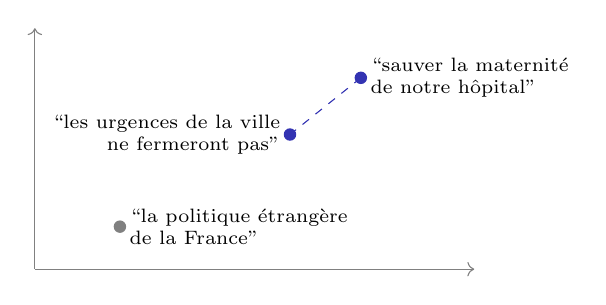
\begin{tikzpicture}[font=\scriptsize,scale=0.9]
  \draw[->,gray] (0,0) -- (6.2,0);
  \draw[->,gray] (0,0) -- (0,3.4);
  \fill[titleblue] (4.6,2.7) circle (2.5pt) node[right,text=black,align=left] {``sauver la maternit\'e\\de notre h\^opital''};
  \fill[titleblue] (3.6,1.9) circle (2.5pt) node[left,text=black,align=right] {``les urgences de la ville\\ne fermeront pas''};
  \fill[gray] (1.2,0.6) circle (2.5pt) node[right,text=black,align=left] {``la politique \'etrang\`ere\\de la France''};
  \draw[dashed,titleblue] (4.6,2.7) -- (3.6,1.9);
\end{tikzpicture}

\vspace{0.3cm}
\raggedright
\small
\begin{itemize}
    \setlength{\itemsep}{3pt}
    \item Each passage of 80 words becomes 384 numbers. Close passages say similar things, with other words, or with OCR errors.
    \item \texttt{multilingual-e5-small}: MIT licence, French included, 470 MB, runs on a CPU. On the cluster: the 4,010 documents in one job.
    \item Not a judgement: a geometry. You still decide what ``close'' means.
\end{itemize}
\end{frame}

\begin{frame}{Three Uses}
\small
\begin{enumerate}
    \setlength{\itemsep}{8pt}
    \item \textbf{Search by meaning.} ``Il faut sauver la maternit\'e de l'h\^opital de notre ville'': the five closest passages in the corpus. Finds what the dictionary misses.
    \item \textbf{A score.} Each document: its passage closest to four examples of local offers. Read as a ranking: the AUC is the probability that a document with a local offer ranks above one without.
    \item \textbf{Features for a classifier.} The document's vector as input, your codes as labels.
\end{enumerate}

\vspace{0.5cm}
\centering
\alert{The examples you choose are a codebook in disguise.}
\end{frame}

\begin{frame}{A Classifier Trained on Your Codes}
\small
A logistic regression: 384 numbers in, the probability of a local offer out, learned from the class's codes.

\vspace{0.4cm}
\textbf{Cross-validation}: five folds; each gold document is predicted by a model that never saw it. The only honest score with so few codes.

\vspace{0.4cm}
\begin{itemize}
    \setlength{\itemsep}{4pt}
    \item Today, about 60 codes: weak, and it shows.
    \item With a few hundred: often as good as an LLM on a narrow concept, for nothing per document.
    \item Your 100 coded texts: notebook Part 7, prompt 12.
\end{itemize}
\end{frame}

\begin{frame}{When the Classical Tools Win}
\footnotesize
\renewcommand{\arraystretch}{1.5}
\begin{tabular}{@{}>{\raggedright\arraybackslash}p{2.4cm}>{\raggedright\arraybackslash}p{2.3cm}>{\raggedright\arraybackslash}p{2.6cm}>{\raggedright\arraybackslash}p{2.6cm}@{}}
\toprule
& \textbf{Dictionary} & \textbf{Embeddings + classifier} & \textbf{LLM} \\
\midrule
Reads & words & meaning & meaning and instructions \\
You need & a word list & a few hundred codes & a codebook, and validation \\
4,010 documents & free, seconds & minutes of GPU & about a dollar, minutes \\
Same answer tomorrow & yes & yes & not guaranteed \\
The text leaves UZH & no & no & yes, unless local \\
\bottomrule
\end{tabular}

\vspace{0.5cm}
\small
On a narrow, lexical concept with millions of texts, start classical. On a fuzzy concept with a few thousand texts, an LLM, validated. In both cases: the same hand codes decide.
\end{frame}

\begin{frame}{Block 2. A Dictionary, Embeddings, a Classifier}
\small
\textbf{I show.} Notebook, Part 3: the list and its score; two false positives; a search; the AUC; the classifier.

\vspace{0.3cm}
\textbf{You do}
\begin{enumerate}
    \setlength{\itemsep}{3pt}
    \item Run Part 3a. Then the exercise: remove a word, add two, rerun.
    \item Part 3b: one search of your own.
    \item Part 3c, once the sheet is filled: \texttt{GOLD\_SHEET\_CSV} in Part 0.
\end{enumerate}

\vspace{0.3cm}
\textbf{We check.} Shared document: your dictionary's precision and recall, before and after; the AUC; the classifier's $\kappa$.

\vspace{0.3cm}
\textbf{In parallel}: prompt 12 on your 100 texts.
\end{frame}

% ============================================================================
\sectionslide{Part 3. Extracting With an LLM}{From a text to a table}

\begin{frame}{Extraction Is Not Classification}
\small
\textbf{Classification}: one label per document. \textbf{Extraction}: a form, filled in from the text.

\vspace{0.4cm}
\renewcommand{\arraystretch}{1.4}
\footnotesize
\begin{tabular}{@{}>{\raggedright\arraybackslash}p{3.4cm}>{\raggedright\arraybackslash}p{6.6cm}@{}}
\toprule
\textbf{Documents} & \textbf{Variables} \\
\midrule
Politicians' biographies & birth year, education, previous offices \\
Bills, amendments & sponsors, dates, articles changed, amounts \\
News articles & events: who, what, where, when \\
Annual reports & revenue, employees, sites \\
Professions de foi & candidate, profession, offices, party, substitute \\
\bottomrule
\end{tabular}

\vspace{0.4cm}
\small
The point: a table you can \textbf{merge} with another dataset. Today, by \textit{d\'epartement} and constituency.
\end{frame}

\begin{frame}[fragile]{The Form Is the Codebook}
\scriptsize
\begin{verbatim}
class Person(BaseModel):
    nom: str
    prenom: str
    sexe: Literal["H", "F", "?"]
    profession: str
    mandats_en_cours: list[str]

class LocalOffer(BaseModel):
    quote: str            # the evidence first,
    present: bool         # then the decision

class Form(BaseModel):
    titulaire: Person
    soutien: str
    suppleant: Person
    local_offer: LocalOffer
\end{verbatim}

\vspace{0.2cm}
\small
Twelve boxes copied from the text, one judged. The model cannot answer outside the form. The schema goes in your appendix, with the instructions.
\end{frame}

\begin{frame}{The Rules That Matter}
\small
From the instructions (notebook, Part 4):
\begin{itemize}
    \setlength{\itemsep}{5pt}
    \item \textbf{Copy, as printed.} Without titles; the French text is authoritative.
    \item \textbf{Empty rather than guess.} An empty field is an answer; an invented value is an error.
    \item \textbf{Who is who.} The candidate, then the substitute. No substitute: empty fields.
    \item \textbf{Now, not before.} Current offices only: not ``ancien maire'', not party positions.
    \item \textbf{OCR.} Read through the errors; never reconstruct what cannot be read.
\end{itemize}

\vspace{0.4cm}
Each rule answers a failure you will see in Block 3.
\end{frame}

\begin{frame}[fragile]{Two Providers, One Form}
\scriptsize
\begin{verbatim}
r = claude.messages.parse(model="claude-haiku-5-5", max_tokens=1500,
        system=INSTRUCTIONS,
        messages=[{"role": "user", "content": text}],
        output_format=Form, thinking={"type": "disabled"})
form = r.parsed_output

r = gpt.responses.parse(model="gpt-6-luna", max_output_tokens=1500,
        instructions=INSTRUCTIONS, input=text,
        text_format=Form, reasoning={"effort": "none"})
form = r.output_parsed
\end{verbatim}

\vspace{0.3cm}
\small
\begin{itemize}
    \setlength{\itemsep}{4pt}
    \item Same instructions, same schema, same price: \$0.10 per million tokens in, \$0.50 out. The 300 documents: about ten cents per model.
    \item Two models that disagree show you where the text is hard.
    \item Every answer appended to a file as it arrives: a rerun never pays twice.
\end{itemize}
\end{frame}

\begin{frame}{Checking an Extraction: Five Outcomes}
\small
Field by field, against the catalogue:

\vspace{0.3cm}
\renewcommand{\arraystretch}{1.4}
\footnotesize
\begin{tabular}{@{}>{\raggedright\arraybackslash}p{2.6cm}>{\raggedright\arraybackslash}p{2.4cm}>{\raggedright\arraybackslash}p{4.9cm}@{}}
\toprule
\textbf{Outcome} & \textbf{Model, catalogue} & \textbf{What to do} \\
\midrule
match & same, same & nothing \\
mismatch & a value, another & read the PDF: who is right? \\
model only & a value, NR & an invention, or a gap in the catalogue? \\
catalogue only & empty, a value & the model missed it, or was told not to guess \\
both empty & empty, NR & nothing \\
\bottomrule
\end{tabular}

\vspace{0.4cm}
\small
Names must be equal. Professions and parties may differ in wording: ``ouvrier surface'' and ``Ouvrier de la surface'', ``PCF'' and ``Parti communiste fran\c{c}ais''.

\vspace{0.2cm}
\centering
\alert{The catalogue is a coder too. A disagreement is a passage to read.}
\end{frame}

\begin{frame}{The Usual Failures}
\begin{itemize}
    \setlength{\itemsep}{7pt}
    \item \textbf{Invented values}: an office nobody mentions, a profession from the context.
    \item \textbf{Who is who}: the substitute's office given to the candidate.
    \item \textbf{Before and now}: ``ancien maire'' as a current office.
    \item \textbf{The shared leaflet}: two candidates on one page, the party of the other.
    \item \textbf{OCR}: a name misspelled by the scan, then copied faithfully.
    \item \textbf{Length}: a long text cut before the model sees the end.
\end{itemize}

\vspace{0.4cm}
\small
None of these raises an error. Only reading finds them.
\end{frame}

\begin{frame}{Block 3. Claude and GPT Against the Catalogue}
\small
\textbf{I show.} Notebook, Part 4: one form, read against its record; then 300 with each model; the table of outcomes.

\vspace{0.3cm}
\textbf{You do}
\begin{enumerate}
    \setlength{\itemsep}{3pt}
    \item Run Part 4. Watch the cost line.
    \item Read five disagreements, with the PDF open.
    \item The offices: the model's 0/1 against the catalogue's.
\end{enumerate}

\vspace{0.3cm}
\textbf{We check.} Shared document: accuracy per field for both models; one disagreement where the catalogue, not the model, is wrong.

\vspace{0.3cm}
\textbf{In parallel}: prompt 13 on documents of your project.
\end{frame}

% ============================================================================
\sectionslide{Part 4. From Labels to an Estimate}{The question we left open}

\begin{frame}{Why Errors Do Not Wash Out}
\small
Errors in a 0/1 label never wash out. Unrelated to X, they \textbf{shrink} the gap. \textbf{Related to X}, they can push it either way.

\vspace{0.4cm}
\textbf{Today}: mayors name their town more often. A model that reads ``Carvin'' as a local offer says yes more often among mayors: the gap is inflated. A dictionary that misses OCR-damaged words misses more in some \textit{d\'epartements} than in others.

\vspace{0.4cm}
\begin{itemize}
    \setlength{\itemsep}{4pt}
    \item 75\% agreement tells you how often the labels are right, not whether the errors are related to X.
    \item Accurate labels still bias a regression; a random gold sample corrects it (Egami et al.\ 2023).
\end{itemize}
\end{frame}

\begin{frame}[fragile]{The Correction}
\small
For each document: the model's label $\hat Y_i$, your hand code $Y_i$ when it was coded ($R_i = 1$), and the probability $\pi$ of being coded.

\[
\tilde Y_i = \hat Y_i + \frac{R_i}{\pi}\,\big(Y_i - \hat Y_i\big)
\]

Then regress $\tilde Y$ on X, as you would have regressed $\hat Y$.

\vspace{0.2cm}
{\scriptsize
\begin{verbatim}
d["pseudo"] = d.claude + d.R / PI * (d.gold.fillna(0) - d.claude)
smf.ols("pseudo ~ local_mandate", data=d).fit(cov_type="HC1")
\end{verbatim}}

\vspace{0.2cm}
\begin{itemize}
    \setlength{\itemsep}{2pt}
    \item Valid whatever the model's errors, if the gold sample is random with known $\pi$.
    \item The same idea: prediction-powered inference (Angelopoulos et al.\ 2023); with the model's confidence, fewer hand codes (Gligori\'c et al.\ 2025).
    \item The price: a wider interval. The price of not trusting the model.
\end{itemize}
\end{frame}

\begin{frame}{Block 4. Naive and Corrected}
\small
\textbf{I show.} Notebook, Part 5: every measure against the class's codes, then the coefficient, naive and corrected, in one figure.

\vspace{0.3cm}
\textbf{You do}: run Part 5, then Part 6, and download the bundle.

\vspace{0.3cm}
\textbf{We check.} Shared document: for Claude, the coefficient naive and corrected, with the intervals. Does the conclusion change?

\vspace{0.5cm}
\textbf{How to read it}
\begin{itemize}
    \setlength{\itemsep}{3pt}
    \item They agree: say so. The referee has a reason to believe the labels.
    \item They disagree: the corrected one is the estimate; the gap is the bias of the labels.
\end{itemize}
\end{frame}

\begin{frame}{What Goes in the Paper}
\begin{enumerate}
    \setlength{\itemsep}{6pt}
    \item The codebook, the schema, the instructions: files, versioned.
    \item The model ID, the date, the settings; the raw answers in the replication files.
    \item The gold sample: how it was drawn, its size, $\pi$, who coded, their agreement.
    \item Every measure against the gold sample.
    \item The corrected estimate, its interval, and the naive one next to it.
\end{enumerate}

\vspace{0.4cm}
\centering
\small
Prompt 14 writes this section with your agent, from your bundle.
\end{frame}

% ============================================================================
\begin{frame}{Debrief}
\textbf{Three screens.} The job's log. Your dictionary, before and after. The figure of Part 5.

\vspace{0.4cm}
\textbf{One question.} Which measure of Y would you print, and what would you put in the appendix to defend it?

\vspace{0.4cm}
\textbf{Before you leave.} Download your bundle (Part 6). Prompts 12 to 14 and the new section of \texttt{template/CLAUDE.md} into your project. Prompt 05, commit.
\end{frame}

\begin{frame}{Next Session: 2 December 2026}
\textbf{Unstructured Data: Audio, Video, and Text}

\vspace{0.3cm}
\begin{itemize}
    \setlength{\itemsep}{4pt}
    \item From a scan or a recording to a text: OCR, transcription, and their errors.
    \item Models that read images and listen to sound.
    \item Your project, in five minutes.
\end{itemize}

\vspace{0.4cm}
\begin{alertblock}{Carry-over question}
Today's OCR got one word in twenty wrong. Which of today's measures suffers most: the dictionary, the embeddings, or the LLM?
\end{alertblock}

\vspace{0.2cm}
{\footnotesize Bring: twenty scanned pages or ten minutes of audio from your project.}
\end{frame}

\begin{frame}{References}
\vspace{0.1cm}
\raggedright
{\scriptsize
Angelopoulos, A.\ N., Bates, S., Fannjiang, C., Jordan, M.\ I.\ and Zrnic, T.\ (2023). Prediction-Powered Inference. \textit{Science} 382(6671).

\vspace{0.12cm}
Archelec. Archives \'electorales du CEVIPOF, Sciences Po. Internet Archive, collection \texttt{archiveselectoralesducevipof}.

\vspace{0.12cm}
Egami, N., Hinck, M., Stewart, B.\ M.\ and Wei, H.\ (2023). Using Imperfect Surrogates for Downstream Inference: Design-based Supervised Learning for Social Science Applications of Large Language Models. \textit{NeurIPS} 36.

\vspace{0.12cm}
Gligori\'c, K., Zrnic, T., Lee, C., Cand\`es, E.\ and Jurafsky, D.\ (2025). Can Unconfident LLM Annotations Be Used for Confident Conclusions? \textit{NAACL}.

\vspace{0.12cm}
Grimmer, J., Roberts, M.\ E.\ and Stewart, B.\ M.\ (2022). \textit{Text as Data: A New Framework for Machine Learning and the Social Sciences}. Princeton University Press.

\vspace{0.12cm}
Laver, M.\ and Garry, J.\ (2000). Estimating Policy Positions from Political Texts. \textit{American Journal of Political Science} 44(3).

\vspace{0.12cm}
Rooduijn, M.\ and Pauwels, T.\ (2011). Measuring Populism: Comparing Two Methods of Content Analysis. \textit{West European Politics} 34(6).

\vspace{0.12cm}
Wang, L., Yang, N., Huang, X., Yang, L., Majumder, R.\ and Wei, F.\ (2024). Multilingual E5 Text Embeddings: A Technical Report. arXiv:2402.05672.

\vspace{0.12cm}
S3IT documentation: \href{https://docs.s3it.uzh.ch}{\texttt{docs.s3it.uzh.ch}}.
}

\vspace{0.2cm}
{\footnotesize Reading for today: Grimmer, Roberts and Stewart (2022), chapters on dictionaries and embeddings; Egami et al.\ (2023).}
\end{frame}

\end{document}
